%!TEX root=../../template.tex
\section{Second Hypothesis}%
\label{sec:second_hypothesis}

The proposed hypothesis was, as explained in
Section~\ref{sec:intro_hypothesis}, that one could obtain a trace gas'
column density between two points by determining this value on both said
points and then subtracting them one from another. Moreover, this was
achievable with the kind of distances that the proposed monitoring
system would be designed to use. To test this, I have setup an
experiment comprising two spectroscopic assemblies. With them, I was
able to test my approach against an active \gls{DOAS} system. The
expected results included similar levels of detected molecules for the
passive and the active systems.

I defined the protocol and divided into measurements, which are
comprised of sets of unitary actions. These actions included not only
the measurements themselves, but also the collection of reference data
for each measurement moment. In order to guide the conduction of the
experiment, both on my behalf and on the volunteer's, a written protocol
was created and made available to participants. This protocol
constitutes an important part of Appendix~\ref{ap:protocol}.

The experiment was conducted in two "runs". The first run took place on
07/06/2021. A slight logistics-related delay complicated matters. The
first measurement was taken at 06:20, some minutes after sunrise.
Although meteorological conditions were optimal and there were no
hassles, work was interrupted at around 08:20, when the battery of one
of the laptops that were being used ran out. Although not enough to make
claims, it was possible to produce some results from these data, namely
concerning passive \gls{DOAS}. These were presented in
Figure~\ref{fig:exp1_no2_density} and their fits in
Figure~\ref{fig:exp1_fit_east} and Figure~\ref{fig:exp1_fit_west}.

The fits themselves show a lot of signal being measured, although
\gls{no2} has less expression than \gls{o4} in most of the
measurements. For the reader's reference, a cross section of \gls{no2}
and \gls{o4} is included in Figure~\ref{fig:no2_cross_section} and
Figure~\ref{fig:o4_cross_section}, already cut to the analysis
wavelength window. This weak fit expression coincides with the trends
displayed on the \gls{no2} density plot. 

QualAR, a Portuguese public initiative to monitor the territory's air
quality, makes its data public and available for consultation at the
initiative's website~\cite{Ambiente2019}. The QualAR chart for the
concentration of \gls{no2} in the closest monitoring station to the
experiment's site is presented in Figure~\ref{fig:qualar_0706}. By
comparing the chart's data and the experiment's data, one can see that
they seem to approximately agree.

\begin{figure}[htpb]
    \centering
    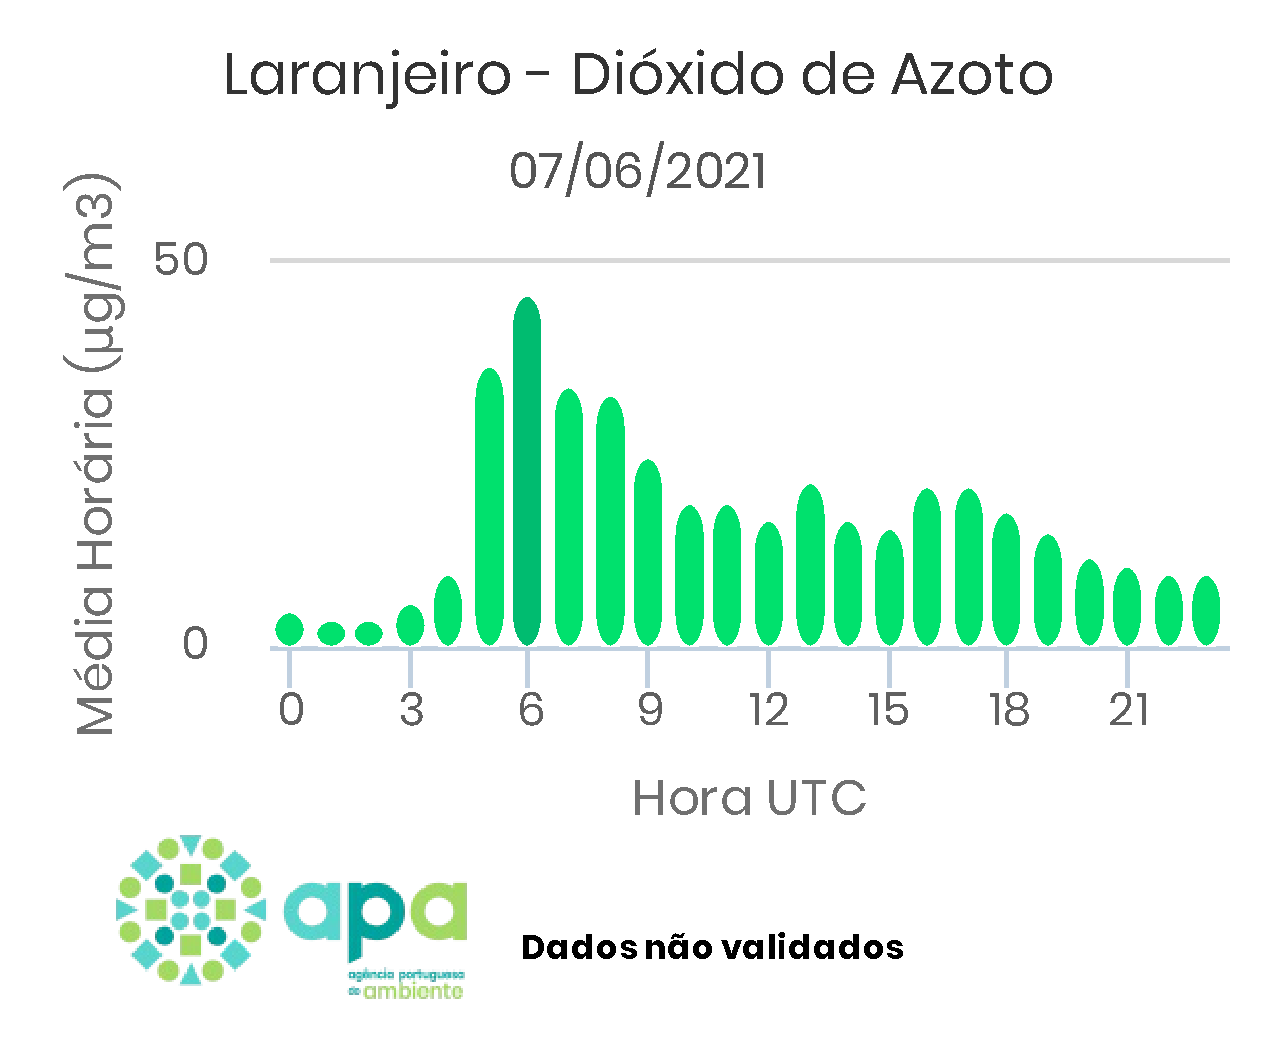
\includegraphics[width=.8\textwidth]{img/pdf/no2_07jun_apa_chart.pdf}
    \caption{QualAR chart for the \gls{no2} concentration at
    the closest monitoring station from the experiment
    site~\cite{Ambiente2019}. 07 June 2021. This chart was directly
    imported from QualAR and is written in Portuguese. The title indicates
    the sampling site (Laranjeiro) and the target gas (Dióxido de Azoto).
    The vertical axis label reads the mean hourly concentration and the
    horizontal one and the horizontal one refers to the hour in \gls{utc}.
    Translation by the author.}
    \label{fig:qualar_0706}
\end{figure}

\begin{figure}[htpb]
    \begin{minipage}{.45\textwidth}
        \centering
        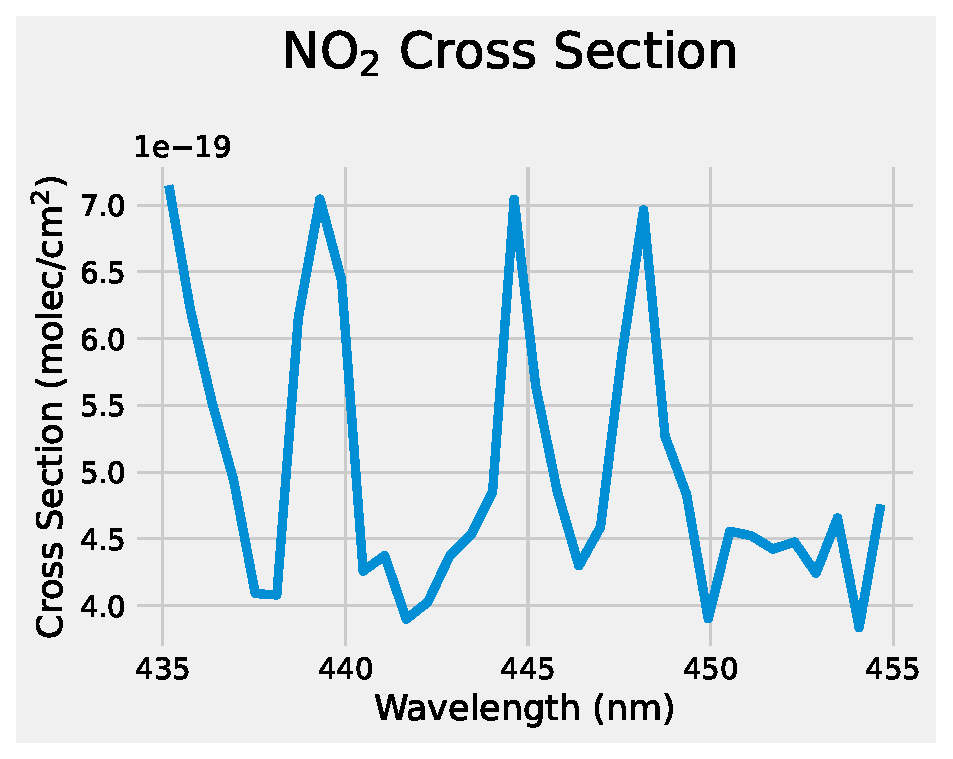
\includegraphics[width=\textwidth]{img/eps/no2_cross_section.eps}
        \caption{Cross section for \gls{no2}, cut to the analysis window
        described in Table~\ref{tab:doas_parameters_exp1}.}
        \label{fig:no2_cross_section}
    \end{minipage}
    \hfill
    \begin{minipage}{.45\textwidth}
        \centering
        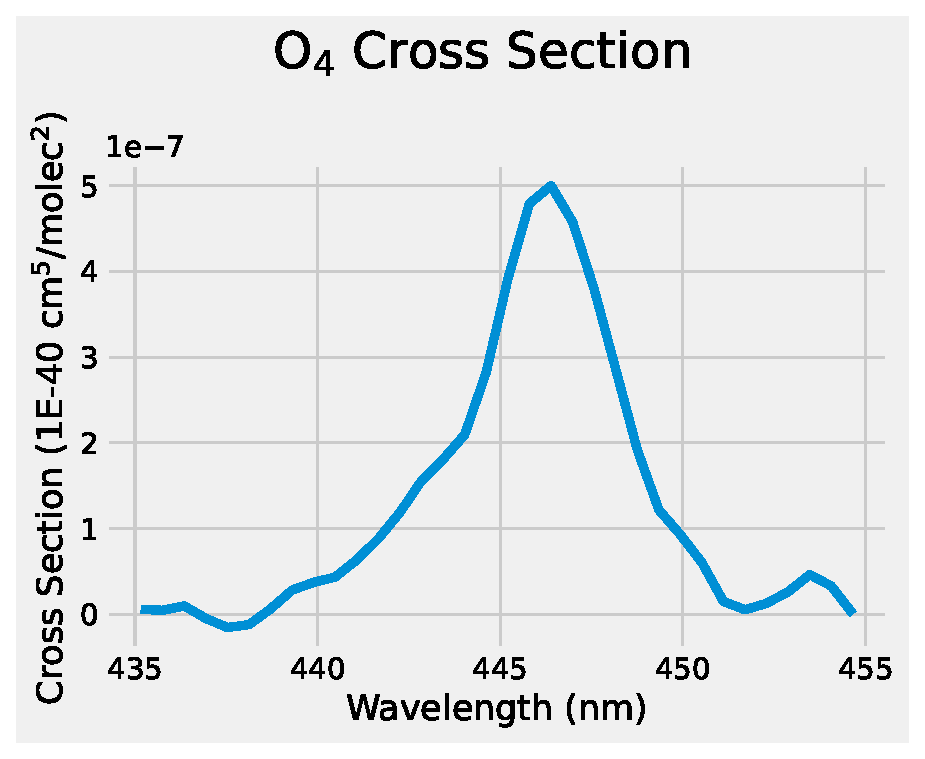
\includegraphics[width=\textwidth]{img/eps/o4_cross_section.eps}
        \caption{Cross section for \gls{o4}, cut to the analysis window
        described in Table~\ref{tab:doas_parameters_exp1}.}
        \label{fig:o4_cross_section}
    \end{minipage}
\end{figure}

The second run of the experiment happened later in the same month, on
the 23\textsuperscript{rd}. The assembly on the East Bank was relocated
around 100m, in an attempt to improve the spectral measurements.
However, this introduced a new challenge. Since the assembly was
positioned farther from the West Bank than in the previous run, the
light source occupied a smaller fraction of the telescope's field of
view. Moreover, in this day we had worse conditions than in the first
day, with wind making the alignment of the two telescopes even more
difficult. In the end, three out of the eleven possible measurements
were discarded due to alignment issues. Coincidentally, the first three.
A relocation schematic is included in
Figure~\ref{fig:changing_position}. There were no logistical problems
this time, and the use of external UPS ensured the laptops would have
sufficient battery to run this experiment until 10:00, half an hour
before the opening of the sanctuary for visitors. 

Again we can analyse the data from two angles:
\begin{description}
    \item[Internal analysis:] did the experiment confirm or deny the
        hypothesis it was meant to test (see
        Section~\ref{sec:second_hypothesis})?
    \item[External analysis:] are the collected data comparable in any
        way with the official data coming from QualAR?
\end{description}

With regards to the first level of analysis, one might initially be
tempted to consider the hypothesis validated if looking only at the
shape of the two plots, Figure~\ref{fig:active_densities} and
Figure~\ref{fig:passive_densities}. They are in fact quite similar in
terms of trend, and they share the same order of magnitude in the scale,
but the values displayed from one to another are quite different. Not so
different as to making the hypothesis implausible, but unfortunately,
not close enough to confirm it directly. As to the fit plots,
Figure~\ref{fig:fit_active}, Figure~\ref{fig:fit_passive_back} and
Figure~\ref{fig:fit_passive_front}, the fit line is much closer to the
signal being fitted (differential optical density) in the passive
experiment than in the active experiment. However, the values of the fit
are one order of magnitude higher in the latter. In every fit, the line
is clearly above noise level, which was one of the most important
concerns in the beginning. 

Regarding the second level of analysis, the official QualAR data are
presented in the chart of Figure~\ref{fig:qualar_2306}. Although this
chart has a low resolution, it is safe to say that the peak value for
\gls{no2} concentration was measured between 07:00 and 08:00. This
contradicts the data collected in the second run of the experiment,
which detected a growing trend for \gls{no2} at least until 10:00. These
differences might be explained with some local effects due to the
proximity of the highway (QualAR's measuring station is near, but in a
completely different surrounding, in the middle of a primary school) or
from some alignment-related instability. 

\begin{figure}[htpb]
    \centering
    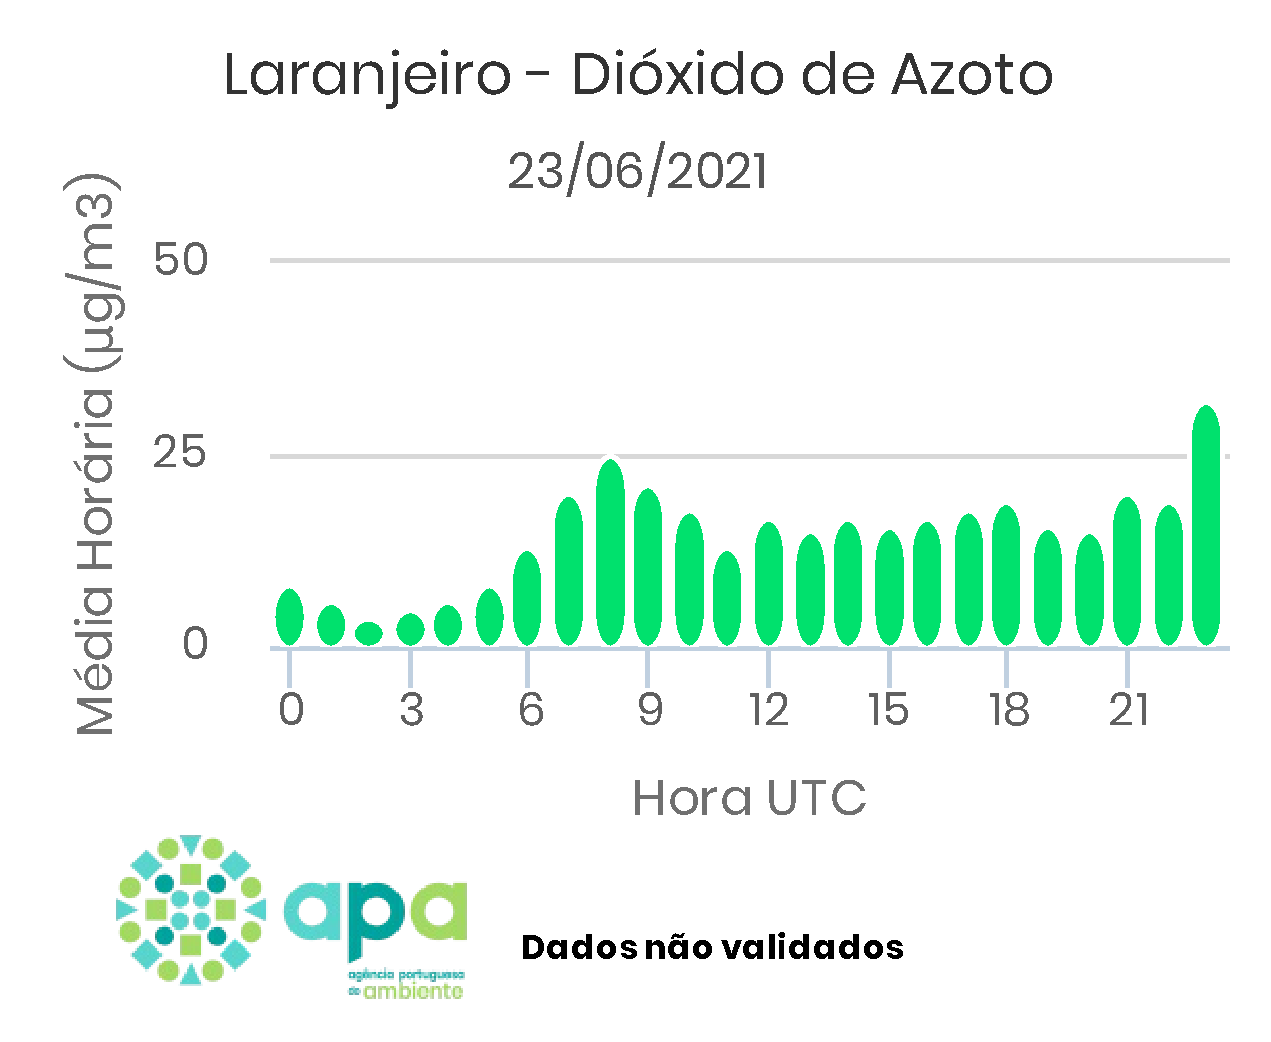
\includegraphics[width=0.8\linewidth]{img/pdf/no2_23jun_apa_chart.pdf}
    \caption{QualAR chart for the \gls{no2} concentration at
    the closest monitoring station from the experiment
    site~\cite{Ambiente2019}. 23 June 2021. This chart was directly
    imported from QualAR and is written in Portuguese. The title indicates
    the sampling site (Laranjeiro) and the target gas (Dióxido de Azoto).
    The vertical axis label reads the mean hourly concentration and the
    horizontal one and the horizontal one refers to the hour in \gls{utc}.
    Translation by the author.}
    \label{fig:qualar_2306}
\end{figure}

Alignment issues are in fact the single most important threat for the
validity of this experiment. As detailed in
Section~\ref{sec:the_experiment}, the experiment was mainly a manual
process, that relied in the sensibility of the two necessarily human
operators to produce the most correct data possible. Given the small
size of the artificial light in the field of view of the telescope, and
the presence of moderately strong winds, this experiment may have been
too tall an order. It is impossible to reach a definite conclusion
without the development of some kind of automatic alignment and
measurement process, that mimics what would be performed by the
autonomous \gls{UAV}.
